\section{Attacco Denial of Service}

\subsection{Definizione}
L'attacco di tipo \textit{Denial of Service} (DOS) consiste nel rendere non disponibili servizi offerti da computer o altri
dispositivi \cite{dos-definition}. Questo avviene esasperando di richieste la macchina o infrastruttura che viene scelta come
vittima. La risorse della vittima verranno quindi interrogate in modo massivo fino al punto di indurre il sistema al collasso.\\
Una variante dell'attacco DOS è il \textit{Distributed Denial of Service} (DDOS), in cui l'attaccante non è composto solamente da una sola
macchina, ma bensì da una rete intera chiamata \textit{botnet}. Questa seconda versione è più difficile da realizzare ma al tempo stesso
molto più efficacie. Solitamente, la \textit{botnet} è composta dagli \textit{zombies}, ovvero dispositivi di utenti normali ignari del fatto 
di essere stati infettati da un \textit{malware} che consente all'attaccante di averne il controllo.\\
\begin{figure}[h]
    \centering
    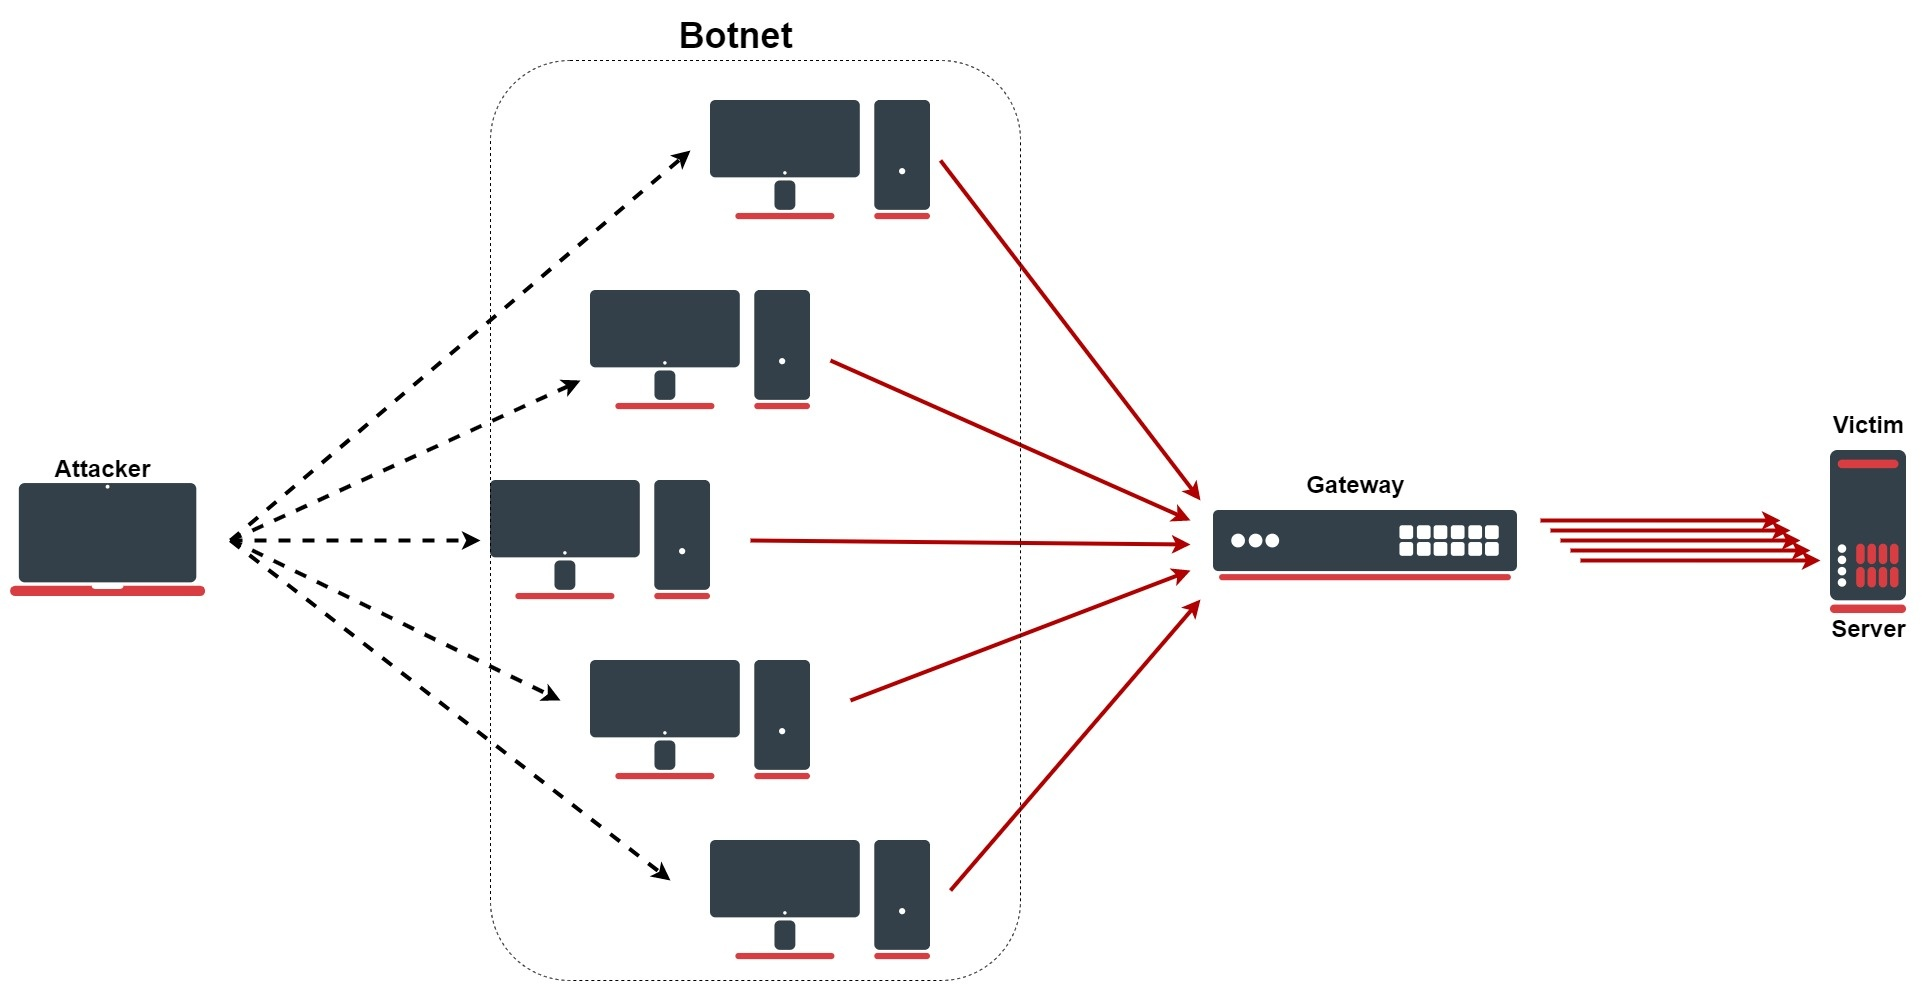
\includegraphics[width=0.5\textwidth]{images/ddos.jpg}
    \caption{Distributed Denial of Service}
\end{figure}

\subsection{Vulnerabilità nelle reti cellulari}
Le reti cellulari non sono esenti da questo tipo di attacchi, anzi, sono una delle tipologie più frequenti e sopratutto difficile da risolvere
poichè le vulnerabilità che sfruttano sono organiche nell'architettura della rete.
Sono diversi i componenti che possono essere vulnerabili a un attacco DOS in una rete cellulare, gli obiettivi identificati come ottimi sono quelli
che comportano un maggior utilizzo delle risorse della rete.\\
Nel caso delle reti cellulari, le maggiori criticità sono rilevate nei meccanismi di identificazione degli utenti, poichè durante queste procedure si
è in grado di interrogare direttamente il \textit{database} che contiene le informazioni degli utenti.
Questo archivio, nel caso delle reti 2G/3G è l'\textit{Home Location Register} (HLR), e rappresenta un punto critico all'interno del \textit{core network}
poichè viene costantemente interrogato per numerose motivazioni come il cambio di posizione del dispotivo connsesso ossia \textit{update location}.
Inoltre, ad aggravare il suo carico di lavoro, è il numero di utenti che deve servire spesso molto alto poichè deve servire aree geografiche molto vaste.

\subsection{Misurazione}
Per capire quale componente della rete sia il più vulnerabile a un attacco DOS si devono fare delle misurazioni sui vari componenti del \textit{network}.
In questo modo è possibile capire in quale punto si possono creare dei rallentamenti o \textit{bottleneck} dovuti a un sovraffollamento di richieste.\\
In \cite{measuring-dos} vi è una dettagliata spiegazione di come procedere con queste misurazioni e sopratutto come quantificare il numero di dispositivi che 
servono all'attaccante per completare l'attacco con successo.